\chapter[Rilevazioni di sub-aloni di DM tramite SGL]{Rilevazioni di sub-aloni di materia \\oscura tramite lensing gravitazionale \\forte}
\label{cap:SGL+DM}
Nei primi due capitoli della tesi, si sono analizzati la materia oscura ed il lensing separatamente, esponendo lo stato dell'arte nei due ambiti. In questo, invece, lo scopo è quello di illustrare come lo strong gravitational lensing possa essere applicato come strumento allo studio della DM, ponendo dei vincoli sui vari modelli teorici tramite le diverse osservazioni. Dapprima verranno presentate in maggior dettaglio le due osservabili principali, ovvero le anomalie nei rapporti di flusso e le perturbazioni alla brillanza superficiale. Successivamente verranno introdotti i modelli utilizzati per descrivere la lente principale e le perturbazioni dei sotto-aloni di materia oscura, ponendo particolare enfasi sulle relative criticità e degenerazioni. Infine, verranno presentati i vincoli attuali forniti dalla letteratura riguardo alle rilevazioni individuali di sotto-strutture, spiegando come essi possano essere usati in un'analisi statistica della popolazione di aloni di materia oscura.
% Vegetti 2024, Strong Gravitational Lensing as a Probe of Dark Matter

\section{Il lensing come strumento di indagine della materia oscura}
I dati raccolti tramite strong gravitational lensing sono sensibili sia a variazioni della distribuzione di materia su scale sub-galattiche all'interno delle galassie lente, sia a quelle lungo la loro linea di vista.
In particolare, ciò che viene modificato è il potenziale della lente e le sue derivate, introdotti nella Sezione \ref{sez:lensing_potential}, che a loro volta influenzano la posizione delle immagini e la magnificazione.
In questa sezione sono descritti brevemente la natura e l'intensità dei principali effetti.

\subsection{Anomalie nei rapporti di flusso}
\label{sez:flux_anomalies}
% Sez. 3
Per modellare il potenziale della galassia lente, generalmente si usano modelli lisci, come il SIE, ai quali viene aggiunto talvolta uno shear esterno per renderli più realistici. Essi permettono di predire le posizioni delle immagini, le magnificazioni ed i rapporti di flusso, secondo le modalità già discusse. Se la massa reale fosse liscia come il modello, allora tali previsioni sarebbero in perfetto accordo con i dati sperimentali. 

Tuttavia, all'interno delle lenti possono essere presenti sub-aloni di massa compresa tra $10^6\ M_\odot$ e $10^9\ M_\odot$, che producono piccole perturbazioni locali del potenziale. Come conseguenza, esse originano generalmente perturbazioni delle posizioni delle immagini piccole rispetto alla scala del sistema macroscopico, mentre possono modificare significativamente le magnificazioni, che dipendono dalle derivate seconde del potenziale. 
Come visto nell'Equazione \ref{eq:magnification}, infatti, la magnificazione è inversamente proporzionale al determinante della matrice $\mathbf{A}$, che a sua volta è legata all'hessiana del potenziale, la quale dipende dalle derivate  seconde.
Poiché l'hessiana indica la curvatura locale del potenziale, anche una piccola massa aggiuntiva può influenzarne significativamente il valore. 

Tali sotto-aloni danno dunque origine ad immagini che sono approssimativamente dove ci si aspetterebbe tramite le predizioni teoriche del modello, ma risultano troppo luminose o, viceversa, troppo deboli; tali incongruenze prendono il nome di \emph{anomalie nei rapporti di flusso}, e permettono di sondare masse inferiori rispetto a quelle direttamente osservabili tramite emissione luminosa.

Da definizione matematica, una \emph{cuspide} (in inglese \emph{cusp}) è un punto in cui si incontrano due rami di una curva che hanno la stessa tangente. Se la caustica presenta delle cuspidi, quando la sorgente vi si avvicina si presenta una configurazione molto particolare sul piano della lente, in cui si formano tre immagini molto ravvicinate fra loro e con magnificazioni elevate; tale configurazione è detta \emph{cusp triplet}. Denominate $A$, $B$ e $C$ le tre immagini, le relative magnificazioni vengono indicate rispettivamente con $\mu_A$, $\mu_B$ e $\mu_C$. A questo punto è possibile definire il parametro adimensionale
\begin{equation}
    R_{cusp}=\frac{|\mu_A+\mu_B+\mu_C|}{|\mu_A|+|\mu_B|+|\mu_C|}
\end{equation}
Poiché la teoria del lensing prevede che, se il potenziale è liscio, $\mu_A+\mu_B+\mu_C \to 0$, tale parametro indica quanto la configurazione osservata si discosta dalla relazione di cuspide prevista per una lente con potenziale perfettamente liscio, ed è normalizzato rispetto alla somma delle magnificazioni assolute, rendendo il parametro indipendente dalla luminosità intrinseca della sorgente.
Nell'intorno di una cuspide, piccole perturbazioni al potenziale gravitazionale producono grandi variazioni nella luminosità, ed è dunque qui che diventa più facile osservare delle anomalie di flusso; inoltre, esse risultano facilmente quantificabili grazie al parametro appena introdotto. 

Un articolo storico sulle anomalie di flusso che sfrutta l'analisi del parametro $R_{cusp}$ è \textcite{Keeton2003}. Gli autori sviluppano una descrizione quantitativa delle anomalie nelle configurazioni cusp, misurando la violazione della relazione di cuspide riportata sopra in termini delle proprietà locali del potenziale di lensing. Essi mostrano che, sebbene $R_{cusp}$ debba tendere a zero nel limite ideale in cui la sorgente si trova esattamente sulla cuspide, valori non nulli sono attesi anche per modelli perfettamente lisci quando la sorgente si trova a distanza finita da essa. Tuttavia, alcune configurazioni osservate presentano valori di $R_{cusp}$ significativamente più grandi rispetto alle predizioni dei modelli lisci realistici, nonostante al loro interno fosse stata inclusa una grande varietà di lenti, comprese galassie con ellitticità, shear esterno e diverse distribuzioni radiali di massa. Un sunto del loro studio viene mostrato graficamente in Figura \ref{fig:flux_ratio_anomalies}.
\begin{figure}
    \centering
    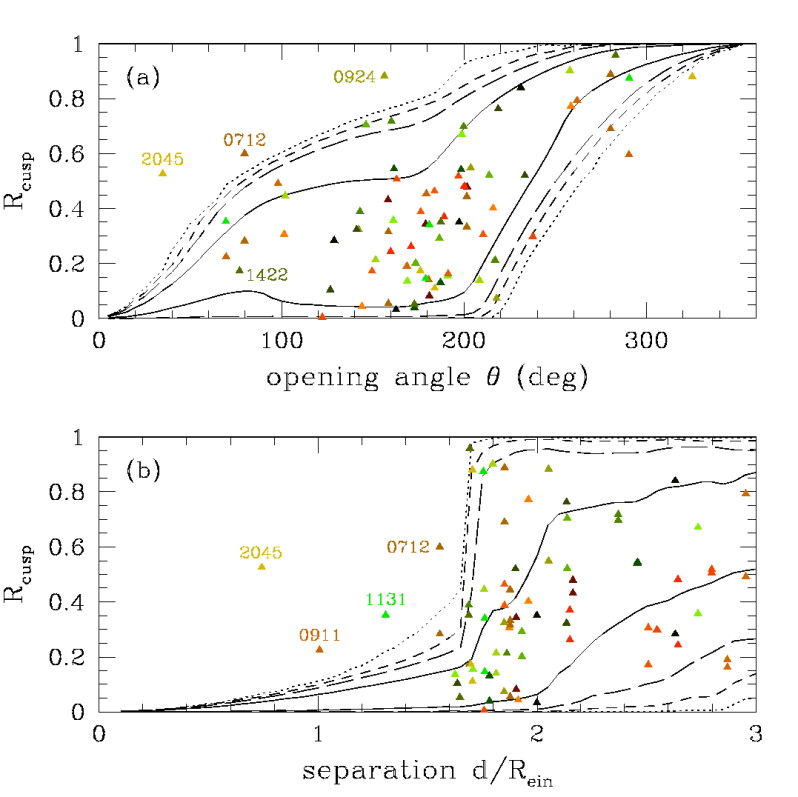
\includegraphics[width=0.9\linewidth]{Immagini/3-DM+Lensing/flux-anomalies.png}
    \caption{Immagine rappresentativa delle anomalie di flusso. Le varie linee indicano contorni di probabilità condizionata costante, ottenuti da simulazioni Monte Carlo. In particolare, esse rappresentano la probabilità di ottenere un certo valore di $R_{cusp}$ dato l'angolo di apertura del tripletto (in alto) o data la distanza normalizzata tra le immagini (in basso). Il livello di confidenza aumenta procedendo dall'interno verso l'esterno; l'ultima curva punteggiata corrisponde al 99.9\%. Il fatto che alcuni punti sperimentali (triangoli colorati) cadano ben al di fuori di qualsiasi contorno indica che la distribuzione di massa liscia della galassia non è sufficiente a spiegare le osservazioni.}
    \label{fig:flux_ratio_anomalies}
\end{figure}
L'incongruenza che emerge tra simulazioni e dati raccolti indica che la distribuzione di massa liscia della galassia non è sufficiente a spiegare le osservazioni, ma ad oggi sappiamo che ciò non indica necessariamente la presenza di sotto-strutture di materia oscura nella galassia lente. Infatti, la presenza di struttura barionica o di aloni lungo la linea di vista crea anomalie simili, pur se causate da strutture a piccola scala differenti.

Le anomalie nei rapporti di flusso sono quindi osservabili che sfruttano la sensibilità della magnificazione alle perturbazioni locali del potenziale, e possono contribuire a porre dei vincoli osservativi all'indagine della DM. Tuttavia, esse sono limitate dalla natura puntiforme delle sorgenti e dalla degenerazione con fenomeni astrofisici non legati alla materia oscura. Un approccio complementare, utile da affiancarvi, consiste nell'utilizzare sorgenti estese, per le quali le perturbazioni si manifestano direttamente come deformazioni della distribuzione di brillanza superficiale.

\subsection{Perturbazioni alla brillanza superficiale }
\label{sez:I_perturbations}
Quando la sorgente non è puntiforme come un quasar, ma piuttosto estesa come una galassia, il numero di informazioni che si possono ricavare dalla deformazione tramite la lente è nettamente maggiore. 

Nel galaxy-galaxy lensing, la sorgente è modellata esattamente allo stesso modo del caso puntiforme, ovvero tramite un modello liscio (tipicamente, anche in questo caso, SIE con l'aggiunta di shear esterno). Tuttavia, quando essa viene deformata dalla galassia lente, ciò che si manifesta non sono più immagini puntiformi, bensì archi gravitazionali e, nella migliore delle ipotesi, interi anelli di Einstein. 
Il numero di pixel che possono essere confrontati fra simulazione e osservazione è dunque superiore.
Inoltre, se vicino ad un arco è presente un sub-alone, esso come visto perturba localmente il potenziale. Di conseguenza, quando la massa è sufficientemente grande si crea una piccola deformazione locale dell'arco; studiando il residuo osservazione-modello è dunque possibile non solo localizzare l'alone, ma anche dedurne la distribuzione di massa (questo perché, come accennato nel Capitolo \ref{cap:cosmologia}, più la distribuzione è concentrata, più efficace è la lente).
Un esempio in cui il satellite presenta anche una controparte visibile è riportato in Figura \ref{fig:visible_satellite}; il satellite è indicato con l'etichetta G4.
\begin{figure}
    \centering
    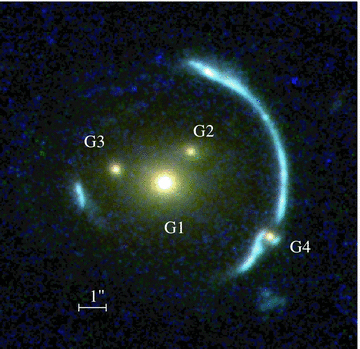
\includegraphics[width=0.5\linewidth]{Immagini//3-DM+Lensing/visible_satellite.png}
    \caption{Esempio di arco gravitazionale deformato localmente da un satellite visibile, denominato con G4. L'etichetta G1 indica la galassia che funge da lente principale, mentre G2 e G3 sono altre due galassie del gruppo. Immagine riprodotta da \textcite{Vegetti2010}.}
    \label{fig:visible_satellite}
\end{figure}

In particolare, ciò che viene confrontato tra osservazioni e simulazioni è la \emph{distribuzione della brillanza} $I(x,y)$, cioè la luminosità in ogni punto dell'immagine: se non esiste un modello liscio capace di riprodurre ogni pixel dell'arco, allora ciò è indice di una mancanza di massa. 
Successivamente, il procedimento consiste nell'introdurre nel modello una piccola perturbazione del potenziale, provando il maggior numero di configurazioni possibili; se una certa posizione e una determinata massa migliorano drasticamente la ricostruzione dell'arco, allora la perturbazione viene interpretata come una sotto-struttura di DM. Esempi di applicazioni alla rilevazione di singole sotto-strutture sono presentati nel paragrafo \ref{sez:indiv_DM_subhaloes}.

Tale metodo risulta essere molto più potente del precedente, ed è fra i più utilizzati negli studi moderni: confrontare migliaia di pixel, infatti, permette di abbattere significativamente le incertezze statistiche rispetto ai pochi flussi precedenti, e dunque le stime della posizione del sub-alone, della sua massa e del suo raggio di scala  risultano molto più precise.
Tuttavia, uno dei limiti delle perturbazioni alla brillanza superficiale è che la massa degli aloni rilevabili dipende fortemente dalla sensibilità degli strumenti di osservazione utilizzati: al di sotto di una certa massa soglia, infatti, gli effetti di deformazione diventano talmente deboli da risultare indistinguibili dall'arco originale; di conseguenza, l'alone diventa invisibile pur rimanendo presente. 
Nonostante ciò, studiare le perturbazioni alla brillanza superficiale è attualmente preferito rispetto alle anomalie di flusso. 

Entrambe le osservabili presentate si basano sullo stesso principio fisico, ovvero sull'identificazione di discrepanze tra le osservazioni e le predizioni ottenute da un modello del sistema di lensing. La costruzione di tale modello e la valutazione delle sue incertezze rivestono dunque un ruolo fondamentale nello studio della materia oscura, poiché determinano la capacità di distinguere le perturbazioni dovute a sotto-strutture massive da eventuali imperfezioni nella descrizione della lente e della sorgente. Per questo motivo, nella sezione successiva vengono approfondite le principali tecniche di modelling utilizzate per descrivere sia la lente principale, sia i sotto-aloni di materia oscura.

\section{Modelling dei sistemi di strong gravitational lensing}

L'analisi dei sistemi di strong gravitational lensing finalizzata alla ricerca di sotto-strutture di materia oscura viene generalmente formulata come un problema di \emph{inferenza bayesiana gerarchica}. 
L'inferenza bayesiana consiste dapprima nel definire un modello parametrico del sistema, che permetta di simulare le osservazioni attese per un dato insieme di parametri. In seguito viene stimata computazionalmente la distribuzione a posteriori di tali parametri; confrontando le osservazioni simulate dal relativo modello con i dati reali, infatti, possono essere ricavati i valori dei parametri più probabili per il sistema e le relative incertezze.
Esistono due livelli principali dell'inferenza: quello relativo ai parametri del singolo sistema in esame e quello relativo agli iperparametri che descrivono la popolazione dei sub-aloni. Il carattere gerarchico consente di combinare le informazioni ottenute da molti sistemi di lensing, con lo scopo di dedurre le proprietà statistiche della popolazione dei sub-aloni; ciò permette dunque di passare dal primo livello al secondo, ed è utile ai fini di distinguere tra loro i diversi modelli di materia oscura.

I parametri del modello sono quantità incognite del sistema e includono la distribuzione di massa della lente principale, le proprietà della sorgente e quelle delle eventuali perturbazioni dei sub-aloni. 
Fra queste, il profilo di massa della lente determina il principale contributo al potenziale gravitazionale; gli aloni, invece, sono perturbazioni locali a tale potenziale. È necessario dunque parametrizzare entrambe le componenti, perché descrivono contributi fisici diversi.  
\newline
\subsection{Modello della lente principale}
La prima componente da inserire nel modello è la distribuzione di massa della lente. Su scala galattica, il principale deflettore è tipicamente una singola galassia massiccia di tipo early-type.
Le parametrizzazioni utilizzate più comunemente per descrivere queste distribuzioni di densità di massa sono un singolo profilo a legge di potenza (\emph{single power law}, SPL) oppure il profilo SIE combinato con uno shear esterno. 

Lo \emph{shear esterno} è un campo che serve per descrivere l'effetto gravitazionale al primo ordine dovuto alla materia circostante alla galassia e alla distribuzione di massa lungo la linea di vista. Esso  permette di sintetizzare gli effetti delle perturbazioni esterne, senza necessariamente distinguerne tutti i contributi, e soprattutto senza aggiungere massa alla lente principale. La distorsione quadrupolare del potenziale gravitazionale introdotta dallo shear modifica le posizioni relative delle immagini, la loro forma e le magnificazioni e influenza dunque le immagini sul piano della lente predette dal modello. 

La scelta di questi specifici profili è motivata dall'analisi di campioni relativamente ampi di galassie lente, che ben vi si adattano.
Tuttavia, la complessità del modello macroscopico rappresenta il limite principale alla capacità di interpretare un residuo come firma di un sub-alone. 
Infatti,  è improbabile che le galassie reali siano semplici oggetti ellittici; al contrario, ci si aspetta che esse abbiano strutture radiali  e angolari più complesse.  Tutte le componenti che vengono trascurate nel modello della lente si riflettono in una potenziale sovrastima o sottostima degli aloni di materia oscura, che possono portare ad inferenze erronee sulle proprietà di quest'ultima.

Una delle criticità che sono emerse nel tempo, per esempio, è la scoperta di componenti a disco in diverse galassie lente che precedentemente erano state considerate puramente ellittiche. Tali dischi, infatti, producono un effetto di lensing non trascurabile, e in alcuni sistemi possono causare delle anomalie di flusso comparabili a quelle attribuite ai subhaloes di DM \parencite{Hsueh2017}. Anche le perturbazioni di multipolo alla struttura angolare delle galassie lente sono una sorgente significativa di falsi positivi nella rilevazione di sub-aloni di masse maggiori \parencite{VegettiORiordan2024}.  Un'ulteriore degenerazione può essere dovuta alla distribuzione della brillanza superficiale della galassia lente, che può talvolta sovrapporsi agli archi e introdurre residui.
Essa viene generalmente sottratta ai dati preventivamente o inferita nel modello usando (tipicamente) un \emph{profilo di Sérsic}
\begin{equation}
    I(r)=I_e e^{-b_n\Big[\Big(\frac{r}{r_e}\Big)^{\frac{1}{n}}-1\Big]}
    \label{eq:Sersic}
\end{equation}
dove $I_e$ è la brillanza superficiale al raggio efficace $r_e$, il quale contiene metà della luminosità totale , $n$ è detto \emph{indice di Sérsic} e controlla il grado di curvatura della funzione e $b_n$ è una costante di normalizzazione che dipende dalla scelta di $n$. Ciò è vero in particolare per le \emph{sorgenti risolte}, ovvero quelle di cui si distingue la struttura spaziale.

In conclusione, la degenerazione tra differenti forme di complessità del potenziale di lensing rappresenta in generale una delle principali fonti di errore sistematico nell'inferenza delle proprietà della materia oscura.  Quando si modella la lente, è fondamentale includere quanti più contributi possibili nella parametrizzazione affinché le rilevazioni degli aloni possano essere considerate attendibili.
Inoltre, i risultati basati su un unico sistema non possono essere generalizzati facilmente ad altri oggetti, in quanto le degenerazioni presenti cambiano in base al campione. 

Una volta individuato con sufficiente confidenza il sub-alone, anch'esso deve essere compreso nel modello e parametrizzato; il modo in cui ciò viene fatto è approfondito nella sezione successiva.

\subsection{Modello dei sub-aloni}
Dopo aver individuato una possibile perturbazione compatibile con la presenza di una sotto-struttura di materia oscura, è necessario introdurla esplicitamente nel modello di lensing. In particolare, è importante porre la propria attenzione sulla scelta della parametrizzazione, in quanto sia la massa totale dell'alone che la sua distribuzione spaziale influenzano l'efficacia della lente.

In letteratura, sono stati sviluppati diversi approcci per descrivere i sub-aloni e, più in generale, tutti gli aloni di piccola massa. Le proprietà da specificare includono la massa, la posizione rispetto alla lente, il redshift ed il profilo di densità, in quanto tutte incidono direttamente sulla deflessione gravitazionale e sulla capacità di rilevare tali sub-aloni durante le osservazioni.

L'approccio più diffuso consiste nel rappresentare anche i sub-aloni con profili di densità parametrici, in perfetta analogia con le lenti. Tuttavia, la forma dei profili scelti è tipicamente differente; tra i più utilizzati vi sono il profilo NFW (Eq. \ref{eq:NFW}) e il profilo Pseudo-Jaffe. 

Nel caso del profilo NFW, la distribuzione di densità è descritta dal raggio di scala $r_s$ e dalla densità di normalizzazione $\rho_s$, che sono caratteristici della struttura e dipendono dal modello di materia oscura utilizzato. In particolare, si richiama che il raggio di scala individua la transizione tra una regione interna in cui la densità decresce approssimativamente come $\frac{1}{r}$ e una regione esterna in cui essa decresce come $\frac{1}{r^3}$. Insieme alla densità caratteristica, esso determina il grado di concentrazione dell'alone.

Il profilo \emph{Pseudo-Jaffe}, invece, è generalmente espresso come differenza di due profili SIS 
\begin{equation}
    \rho(r)=\frac{\sigma_v^2}{2\pi G}\Big(\frac{1}{r^2}-\frac{1}{r^2+r_t^2}\Big) 
\end{equation}
dove $\sigma_v$ è la dispersione di velocità del sub-alone, mentre $r_t$ è detto \emph{raggio di troncamento}. Analogamente al raggio di scala del profilo NFW, esso identifica una scala caratteristica della distribuzione di massa; a differenza di $r_s$, tuttavia, il raggio $r_t$ introduce un vero e proprio troncamento del profilo. 
Per $r\ll r_t$, infatti, si ha 
\begin{equation}
    \rho(r) \propto \frac{1}{r^2}
\end{equation}
che è l'andamento del SIS e risulta più ripido rispetto al NFW nelle zone centrali. Per $r\gg r_t$, invece, l'andamento è 
\begin{equation}
    \rho(r) \propto\frac{1}{r^4}
\end{equation}
Esso permette alla massa totale di rimanere finita anche per raggi infiniti, in quanto decresce più rapidamente di un classico profilo NFW. 

Il profilo di Navarro, Frenk e White viene generalmente usato per descrivere aloni isolati, che possono influenzare il potenziale anche a grandi distanze; il troncamento del profilo Pseudo-Jaffe, invece, descrive particolarmente bene i sub-aloni, perché include gli effetti dello stripping mareale dell'alone ospite, che agisce sulla parte più esterna sottraendo massa. Esso permette anche di semplificare i calcoli analitici del lensing. 

Nei modelli più completi, il numero di aloni e sub-aloni lungo la linea di vista viene estratto da distribuzioni statistiche basate sulla relativa funzione di massa. Le loro posizioni proiettate, invece, sono assegnate secondo distribuzioni spaziali motivate dalle simulazioni cosmologiche. Dopo aver definito tali proprietà, il contributo dei singoli aloni al potenziale gravitazionale totale può essere calcolato in maniera diretta e sommato al contributo della lente principale, il quale viene modellato come descritto nella sezione precedente. 

Oltre ai modelli parametrici, esistono approcci più flessibili in cui i sub-aloni non vengono descritti individualmente. Tra di essi figurano i modelli pixellati, in cui le sotto-strutture sono rappresentate come correzioni locali del potenziale gravitazionale senza ulteriori assunzioni sul numero di aloni o sul loro profilo di densità, e il \emph{Gaussian Random Field} (GRF, campo gaussiano randomico), che modella le fluttuazioni statistiche complessive del campo di densità e da cui è possibile inferire le proprietà della popolazione di aloni. Tali metodi non saranno approfonditi in ulteriore dettaglio, in quanto esula dallo scopo di questa tesi. 

Le differenti strategie di modelling descritte in queste sezioni costituiscono la base metodologica per l'interpretazione delle osservazioni di strong lensing. Definito il modello della lente e delle eventuali sotto-strutture è infatti possibile confrontarne le predizioni con i dati osservativi, ricavando così i vincoli quantitativi cercati sulle proprietà della materia oscura. Nella sezione seguente vengono presentati i principali risultati ottenuti in letteratura, sia attraverso rilevazioni individuali che mediante analisi statistiche.
\newline
\section{Vincoli attuali della letteratura}
A livello osservativo, esistono due  principali tipi di sorgenti coinvolte nei sistemi di strong gravitational lensing: le \emph{sorgenti irrisolte}, ovvero puntiformi, in cui le informazioni principali sono ottenibili tramite la posizione ed il flusso delle immagini multiple, e le \emph{sorgenti risolte}, ovvero estese, in cui è possibile analizzare la struttura superficiale degli archi e degli anelli pixel per pixel. 
Entrambe risultano essere di fondamentale importanza nello studio della materia oscura, in quanto complementari fra loro: le sorgenti irrisolte sono più frequenti da osservare e molto sensibili agli aloni di piccola massa, ma sono anche più soggette a degenerazioni dovute alla complessità del modello e al microlensing; le sorgenti risolte, invece, sono più rare, ma permettono di ottenere vincoli più robusti sulla DM, in quanto grazie alla maggiore quantità di informazioni ottenibili è possibile distinguere le diverse componenti di massa coinvolte. Tuttavia, esse richiedono anche risoluzioni  angolari molto elevate.
In questo paragrafo si pone particolare attenzione alle sorgenti risolte, in quanto esse permettono, in linea di principio, di distinguere le strutture intrinseche della sorgente dalle perturbazioni locali del potenziale; i vincoli sulla DM sono dunque dedotti con maggiore confidenza.

Individuata la sorgente è poi possibile avere tipi diversi di rilevazioni.
Se la rilevazione è \emph{individuale}, viene identificata un'anomalia in un singolo sistema e la si interpreta come un possibile sub-alone. Tuttavia, dato il carattere gerarchico dell'inferenza dei modelli, è possibile porre anche \emph{vincoli statistici}, considerando una popolazione numerosa di sistemi e deducendo proprietà collettive come  la normalizzazione della funzione di massa, la sua pendenza o lo spettro di potenza delle strutture su piccola scala. Tali informazioni permettono poi di confrontare i vari modelli teorici di materia oscura e discernerli tra loro. Nel seguito, verranno approfonditi entrambi gli approcci in relazione alle sorgenti risolte.

\subsection{Rilevazioni individuali di sub-aloni}
\label{sez:indiv_DM_subhaloes}
La prima rilevazione di una galassia satellite nana al di fuori dell'Universo Locale, ottenuta unicamente tramite effetto gravitazionale, è descritta nell'articolo \textcite{Vegetti2010}.  In particolare, gli autori hanno individuato una sotto-struttura oscura, precedentemente passata inosservata dall'immagine di HST, nella galassia lente SDSSJ0946+1006, appartenente al campione SLACS e più comunemente conosciuta come \emph{Double Einstein Ring}. Tale rilevazione, avvenuta mediante imaging gravitazionale diretto, è stata poi confermata modellando la sotto-struttura con una variazione del profilo di densità Pseudo-Jaffe. Tramite tale modello, si è stimato che la struttura avesse una massa pari a $M_{sub}=(3.51 \pm 0.15)\cdot 10^9\ M_\odot$ e fosse localizzata esattamente nella posizione in cui la mappa di densità superficiale mostrava un marcato picco di convergenza.

\begin{figure}
    \centering
    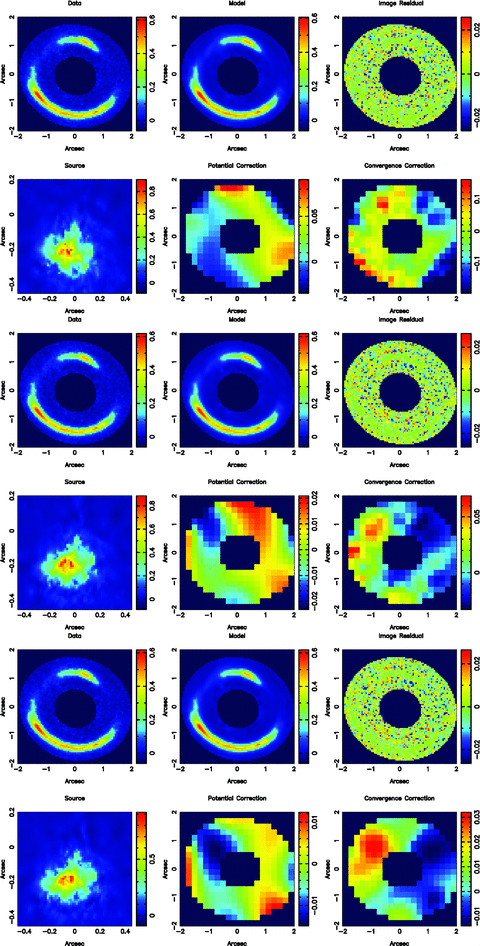
\includegraphics[width=0.7\linewidth]{Immagini//3-DM+Lensing/Vegetti2010.png}
    \caption{Risultato della ricostruzione pixellizzata della sorgente e delle correzioni al potenziale della lente per tre diversi valori del parametro di regolarizzazione $\lambda_{\delta\psi}$ (dall'alto verso il basso, $10^7, 10^8, 10^9$). Il pannello in alto a sinistra mostra i dati originali della lente, quello centrale la ricostruzione finale del modello e quello in alto a destra i residui delle immagini. Nella seconda riga, invece, da sinistra verso destra, sono mostrate rispettivamente la ricostruzione della sorgente, la correzione al potenziale e la convergenza associata alla correzione del potenziale. Immagine riprodotta da \textcite{Vegetti2010}.}
    \label{fig:Vegetti 2010}
\end{figure}
In Figura \ref{fig:Vegetti 2010} sono mostrate diverse ricostruzioni della sorgente e delle correzioni del potenziale della lente per valori crescenti del parametro di regolarizzazione, ottenute tramite imaging gravitazionale diretto. Sebbene la presenza della sotto-struttura non sia osservabile direttamente nei dati originali, essa diventa particolarmente evidente quando si analizza la convergenza associata alla correzione del potenziale, in quanto essa presenta un picco localizzato (rappresentato in rosso in figura) sempre più accentuato.

Una seconda rilevazione di satellite oscuro in una galassia lente early-type tramite gravitational lensing è descritta nell'articolo \textcite{Vegetti2012}.
Gli autori, seguendo un procedimento simile a quello dell'articolo precedente, riportano la presenza di una galassia satellite oscura di massa $M=(1.9 \pm 0.1) \cdot 10^8\ M_\odot$ nel sistema Einstein ring JVAS B1938+666. Tale sistema è un candidato eccellente per la ricerca di perturbazioni alla brillanza superficiale, in quanto presenta un anello di Einstein quasi completo e fortemente amplificato; di conseguenza, la presenza della galassia satellite introduce una perturbazione localizzata nell'arco originario. Il sistema è stato osservato a due diverse lunghezze d'onda nel vicino infrarosso, mediante l'ausilio di ottiche adattive, dal telescopio Keck.  Per il modello di massa totale si è utilizzata una legge di potenza ellissoidale, il cui best fit è stato poi raffinato da correzioni locali del potenziale definite su una griglia regolare. 
\begin{figure}
    \centering
    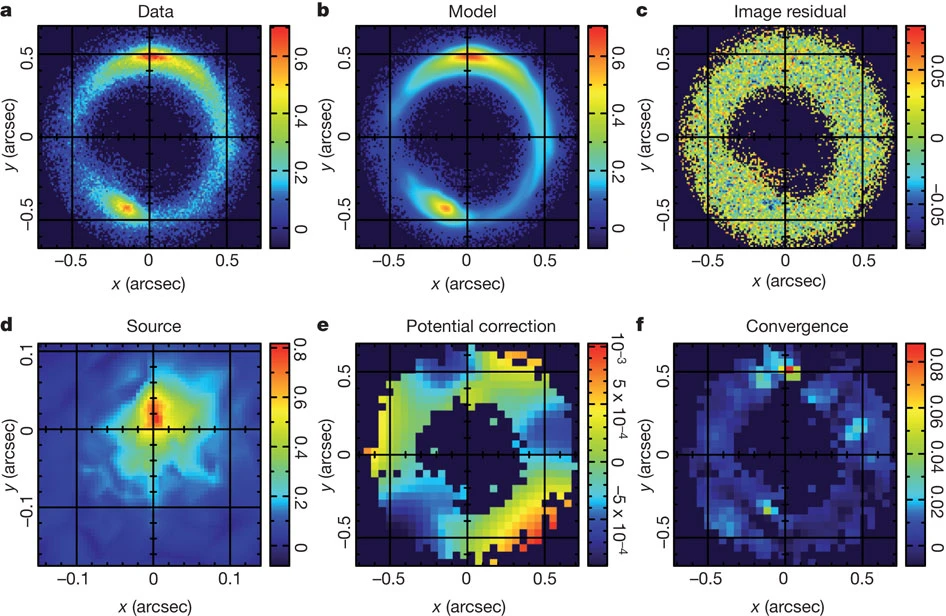
\includegraphics[width=0.8\linewidth]{Immagini//3-DM+Lensing/Vegetti2012.png}
    \caption{Dati ottenuti dal telescopio Keck del sistema JVAS B1938+666 (pannello a), ricostruzione finale del modello (pannello b), residui dell'immagine (pannello c), ricostruzione della sorgente (pannello d), correzione del potenziale (pannello e) e corrispondenti correzioni della densità superficiale proiettata (pannello f). Nella parte superiore dell'arco sottoposto a lensing viene rilevato un picco localizzato, similmente a quanto accadeva nel sistema SDSSJ0946+1006. Immagine riprodotta da \textcite{Vegetti2012}.}
    \label{fig:Vegetti2012}
\end{figure}
Anche in questo caso, come nel precedente, è possibile osservare un picco localizzato nella mappa della convergenza associata alla correzione del potenziale; tuttavia, a differenza del caso precedente, esso corrisponde ad un punto di flusso elevato associato ai dati, ed ha dunque una controparte osservativa.

Lo stesso sistema è stato recentemente oggetto di una nuova rilevazione nell'articolo \textcite{Powell2025}. Essa risulta particolarmente sorprendente, in quanto si riporta la scoperta di un oggetto di massa estremamente bassa, almeno due ordini di grandezza in meno rispetto agli articoli precedenti, individuato attraverso la sua perturbazione gravitazionale su un arco sottile sottoposto a lensing. L'oggetto è stato identificato tramite una tecnica di imaging non parametrica, poi confermato tramite un modello parametrico indipendente. La massa stimata dell'oggetto è pari a $m_{80}=(1.13\pm0.04)\cdot 10^6 \ M_\odot$. Quando l'articolo è stato pubblicato, questo era l'oggetto di massa più bassa mai rilevato a distanza cosmologica attraverso il suo effetto gravitazionale.
\begin{figure}
    \centering
    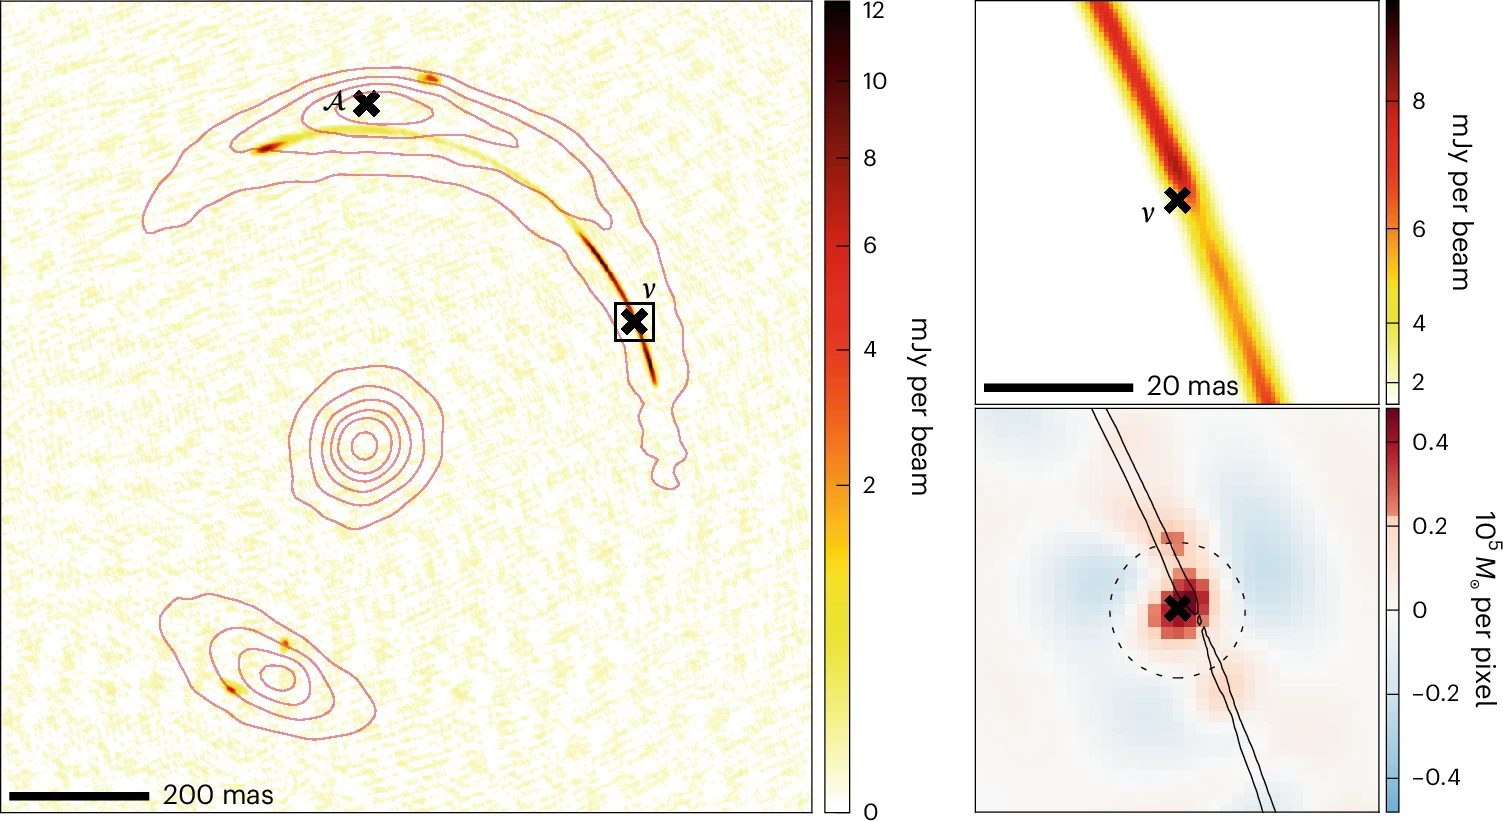
\includegraphics[width=0.8\linewidth]{Immagini//3-DM+Lensing/Powell2025a.png}
    \caption{Ricostruzione più recente del sistema JVAS B1938+666. A sinistra si osserva il miglior modello di brillanza superficiale, in cui sono indicate le due posizioni dei perturbatori con una croce nera; in particolare, $\mathcal{A}$ è l'alone già individuato in \textcite{Vegetti2012}, mentre $\mathcal{V}$ è la nuova scoperta. Nei pannelli laterali si possono osservare il gap nell'arco prodotto dalla perturbazione gravitazionale di $\mathcal{V}$ (in alto a destra) e la mappa di convergenza associata alle correzioni del potenziale gravitazionale (in basso a destra). Immagine riprodotta da \textcite{Powell2025}.}
    \label{fig:Powell2025a}
\end{figure}
In Figura \ref{fig:Powell2025a} è riportata la ricostruzione più recente del sistema. Oltre alla galassia oscura individuata già dodici anni prima e indicata con $\mathcal{A}$, la nuova tecnica di \emph{Very Long Baseline Interferometry} (VLBI) ha mostrato la presenza di un secondo perturbatore più piccolo, indicato con $\mathcal{V}$. L'oggetto è stato confermato utilizzando un confronto con un modello Pseudo-Jaffe.

Ciò che si nota seguendo il filo conduttore di quindici anni di rilevazioni individuali è che, per le sorgenti risolte, è di fondamentale importanza costruire telescopi con una risoluzione angolare sempre maggiore. Il passaggio da HST, a Keck AO (ovvero con \emph{adaptive optics}, ottiche adattive) e infine al più recente VLBI ha permesso di scoprire strutture nuove sempre meno massicce, permettendo di abbattere il limite di massa osservabile di conseguenza. Poter rilevare strutture oscure sempre più piccole, come anticipato nel Capitolo \ref{cap:cosmologia}, permette di vincolare le proprietà della materia oscura, distinguendo tra i diversi modelli teorici che proprio in questa regione presentano previsioni discordanti. Nella sezione successiva, si riprenderanno le stesse rilevazioni e inseriranno nel contesto di campioni più ampi, per analizzarne i vincoli statistici sulla popolazione degli aloni di DM.

\subsection{Vincoli statistici sui modelli di DM}
Finora, nei vari articoli analizzati erano state presentate caratteristiche proprie del singolo alone, come la sua massa o la posizione proiettata sul piano della lente.  Tuttavia, il gran numero di pixel a disposizione per le sorgenti risolte permette di fare una prima inferenza sugli iperparametri della popolazione di cui questi aloni fanno parte.
In particolare, generalmente quando si effettua la rilevazione di un nuovo sistema si stimano due parametri: la frazione di massa contenuta all'interno dell'anello di Einstein costituita da sotto-strutture di DM, denotata con $f$, e la pendenza della legge di potenza che, in prima approssimazione, descrive il numero di strutture attese per unità di massa, ovvero il parametro $\alpha$ dell'Equazione \ref{eq:dn/dM}.  

A seguito della prima rilevazione di una struttura oscura tramite strong gravitational lensing \parencite{Vegetti2010}, si era ottenuto, per l'anello più interno, $f_{CDM}=2.15^{+2.05}_{-1.25} \% $ nel range di massa tra $4\cdot10^6\ M_\odot$ e $4\cdot10^9\ M_\odot$, fissando $\alpha$ a $1.9 \pm 0.1$, in quanto valore ottenuto nella maggior parte delle simulazioni cosmologiche \LCDM.  Gli autori hanno poi realizzato una seconda stima, in cui hanno permesso ad $\alpha$ di variare in un range più ampio, in particolare tra $1.0$ e $3.0$. In questo secondo caso, la percentuale è salita a $f_{CDM}=2.56^{+3.26}_{-1.50} \% $, ma si noti che è salita anche l'incertezza associata. Ciò implica che la stima della frazione di massa corrispondente alle sotto-strutture dipende in maniera non trascurabile dall'assunzione teorica su $\alpha$, e non solo dai dati osservati. Le simulazioni \LCDM \ prevedono un valore pari a $f_{CDM}=0.3 \%$, ovvero circa un settimo di quanto stimato dalla rilevazione. Tuttavia, data l'ampiezza delle barre di errore, il valore ottenuto tramite le simulazioni ha una \emph{likelihood} pari a circa la metà di quella del best-fit osservato; ciò implica che il best-fit, pur non essendo favorito, è plausibile in un Universo dominato dalla materia oscura fredda. 

Quando, due anni dopo, si è scoperto un secondo sistema di massa inferiore \parencite{Vegetti2012}, combinando i dati presentati in precedenza con quelli nuovi si è ottenuta una frazione di sotto-strutture media pari a $\langle f \rangle = 3.3^{+3.6}_{-1.8} \%$  e una pendenza di  $\alpha=1.1^{+0.6}_{-0.4}$ . Tali valori sembrano indicare due discrepanze distinte. Il fatto che $f$ sia superiore al valore previsto di $0.3\%$ indica che, a distanze cosmologiche, la frazione di massa contenuta in sotto-strutture potrebbe essere maggiore di quanto atteso. Il fatto che il valore di $\alpha$ sia minore di $1.9$, invece, potrebbe indicare che la popolazione è meno dominata dalle masse piccole di quanto preveda lo standard \LCDM. Ciò potrebbe essere indice di una componente non trascurabile di WDM, che abbia in parte soppresso le strutture più piccole. In ogni caso, i risultati ottenuti sono consistenti al 95\% con quanto atteso dalle simulazioni standard, indicando un buon accordo di base e confermando la formazione gerarchica delle strutture.

Come sottolineato da \textcite{Powell2025}, le osservazioni su scale sub-galattiche non hanno finora fornito una conferma definitiva del modello \LCDM, principalmente a causa della complessa interazione non lineare tra materia barionica e materia oscura, come descritto in maniera estesa nella Sezione \ref{sez:small_scale_problems}.
Le principali discordanze e tensioni tra i modelli, infatti, si hanno per masse al di sotto delle $10^8\ M_\odot$ , ovvero su piccola scala. In questo contesto, se la struttura di $10^6\ M_\odot$ rilevata fosse realmente un alone di DM (e nell'articolo gli autori spiegano meglio quali sono le alternative plausibili e perché le ritengono meno probabili), essa potrebbe risultare fondamentale nell'indagine sulla materia oscura.
La sua presenza, infatti, sarebbe coerente con il numero atteso di aloni rilevabili in una cosmologia \LCDM: considerando una piccola zona attorno alle immagini lensate, di grandezza paragonabile alla risoluzione strumentale, la probabilità di osservarvi un grumo di materia oscura fredda è infatti pari al $65\%$. Per la WDM, a seconda della massa della particella prodotta termicamente, la probabilità scende a $36\%$ per le particelle più pesanti (di massa pari a $9.1$ keV), che si comportano in modo simile alla CDM, e ancora a $14\%$ per le particelle più leggere (di massa pari a $4.6$ keV), coerente con la  soppressione degli aloni di piccola massa che ci si aspetta per questa tipologia di materia oscura. Sebbene la rilevazione sia dunque compatibile con entrambi i modelli teorici, la probabilità di osservare un alone tanto piccolo è favorito in uno scenario di CDM prevalente e rappresenta un vincolo indipendente rispetto ai parametri $f$ e $\alpha $ presentati in precedenza.

In conclusione, lo strong gravitational lensing risulta essere uno strumento potente: esso, in linea di principio, permette di inferire e rilevare la presenza di oggetti che, non emettendo radiazione elettromagnetica, non sarebbero osservabili direttamente attraverso la loro brillanza superficiale. Tuttavia, come si è cercato di mostrare in questo capitolo, la firma dei sotto-aloni di materia oscura non è sempre netta; poiché entrano in gioco molteplici variabili e interazioni complesse tra di esse, è importante comprendere, attraverso simulazioni di sistemi controllati, come la presenza di un perturbatore modifichi le quantità osservabili. Nel prossimo capitolo, il problema reale di \emph{Bayesian inference} verrà dunque ricondotto a un problema di \emph{forward modelling}, nel quale le proprietà del perturbatore sono fissate a priori e si calcolano le conseguenti modifiche alle osservabili del sistema di lensing, seguendo un filo logico contrario rispetto a quanto si fa normalmente con le osservazioni. 